\documentclass[../main.tex]{subfiles}
\graphicspath{{resources/}{resources/irodalom_res/}}
 
\begin{document}

\section{Okos LED-rendszerek felkutatása, forgalomban lévő eszközök áttekintése}
    Az evolúció során az emberi szem úgy fejlődött ki, hogy nappali fényhez - világoshoz - gyorsan alkalmazkodik, és éles képet alkot. Sötéthez, szürkülethez csak lassan képes alkalmazkodni és akkor sem éles az a kép, amit látunk. A fejlődő világunkban nélkülözhetetlenné vált a világítás, hogy napnyugta után sem álljon meg az élet és tovább tudjuk folytatni tevékenységeinket.

    
    % \begin{figure}[h!] %https://pixabay.com/en/city-night-lights-cityscape-urban-1967190/
    %     \centering
    %         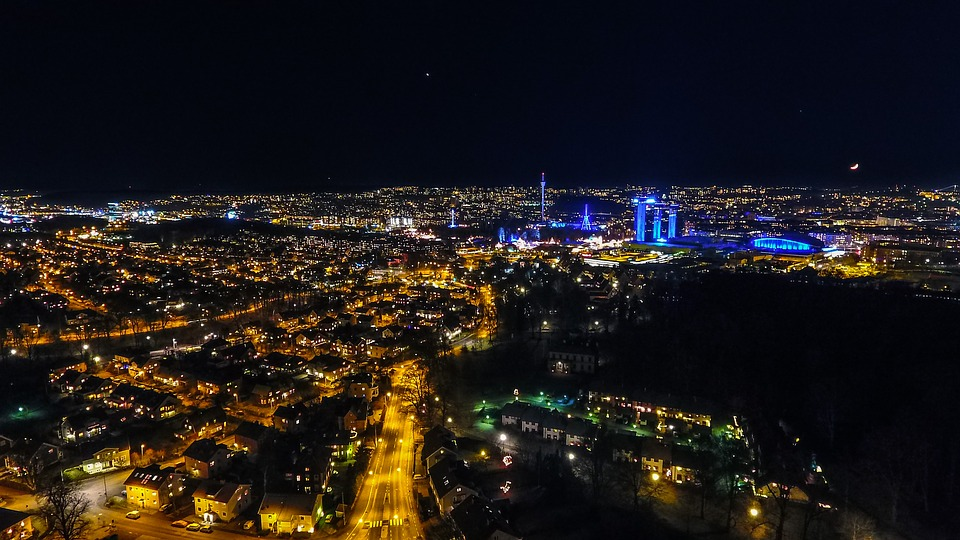
\includegraphics[height=7cm]{irodalom_res/night_life.jpg}
    %     \caption{Éjszakai város látképe} %cite{}
    % \end{figure}
    
    Az általam készített termékkel főként háztartásokban lévő okos világítás megvalósítása a cél, minél energia-gazdaságosabb módon. Erre a legmegfelelőbb technológia a LED világítás\cite{a_energy_efficien_smart_led_systems}.
    
    \subsection{LED világítás és előnyei} 
    A fényt kibocsájtó diódák (angolul: light-emitting diode - LED) a mai legenergiatakarékosabb és leggyorsabban fejlődő világítástechnológiák közzé tartoznak. Általánosságban igaz az, hogy a LED-es izzók tovább bírják, ellenállóbbak és hasonló vagy még jobb minőségű megvilágítást biztosítanak, mint más fényforrások. \citep{led_lighting} 
    
    % \begin{figure}[h!] %https://en.wikipedia.org/wiki/Light-emitting_diode
    %     \centering
    %         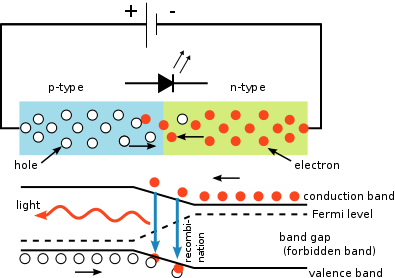
\includegraphics[height=6cm]{irodalom_res/led_working_principle.png}
    %     \caption{LED működési elve - angolul} %cite{}
    % \end{figure}
    
    A következőkben a LED-es világítások előnyeit foglaltam össze.
        \subsubsection{Energiatakarékosság} 
            A LED-es izzók legalább 75\%-kal kevesebb energiát használnak és 25x hosszabb ideig bírják, mint a hagyományos izzólámpák. A LED-es izzók elterjedése lenne az egyik legnagyobb hatással az energiatakarékosságra. Az USA-ban például ezzel 2027-ig 348 $TWh$ elektromos munkát (egy éves teljesítménye 44, egyenként 100 Megawattos erőműnek) spórolhatnánk meg, ahhoz képest, mintha nem használnánk egyáltalán LED-es izzókat, ami több mint 30 milliárd dollár lenne.
            
            A hagyományos izzók teljes teljesítményének 90\%-ából hő termelődik, ami azt jelenti, hogy csak 10\%-a fordítódik fénykibocsátásra. A LED-ek esetében alig termelődik hő. \citep{led_lighting}
        \subsubsection{Jó színvisszaadás}
            A színvisszaadási index, röviden 'CRI' (Color Rendering Index), a fényforrás azon képességét méri, hogy különféle tárgyakat megvilágítva vele, mennyire képes azok színét visszaadni. \citep{led_lighting2}
             \begin{figure}[h!]
                \centering
                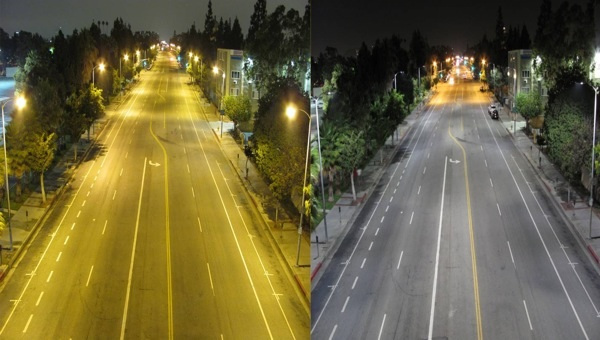
\includegraphics[height=6cm]{irodalom_res/cri_los_angeles.jpg}
                \caption{Utcai megvilágítás kisnyomású nátriumlámpával és LED-del \cite{led_lighting3}}
             \end{figure}

             
        \subsubsection{Környezetbarát}
            A higanylámpával és a fénycsővel ellentétben, a LED-es megoldások nem tartalmaznak higanyt.
        \subsubsection{Széles működési tartomány}
            A LED-ek hidegben és melegben is egyaránt jól funkcionálnak, működésükhöz esetekben nagyon kis feszültségek is elegendők, ezáltal alkalmasak kültéri megvilágításokra is.
    
    \subsection{Forgalomban lévő eszközök áttekintése}
        Manapság rengeteg gyártó kínál okos világítás rendszereket. %, amelyek közül szeretnék bemutatni egy párat, illetve hogy miért érdemes alkalmazni őket. 
        Az okos égők nem csak átlagos LED lámpák, amiket a foglalatba lehet tekerni. Okkal hívják őket okos izzóknak. Vezeték nélkül csatlakoztathatók mobiltelefonjainkhoz vagy Smart Home rendszerünkhöz (Amazon Echo, Google Home), ezzel korlátlan lehetőséget létrehozva. 
        
        Szinte minden ilyen fényforrásnak lehet állítani a fényerősségét anélkül, hogy bármiféle fényerősségszabályzó kapcsolót kéne a falba szerelni. Bárhonnan vezérelhetők, illetve be- és kikapcsolási rutinok állíthatók be rajtuk. Ez például egy nagyszerű biztonsági funkció, mert amikor nyaralni vagyunk, akkor annak a látszatát kelti, mintha otthon lennénk. A ház elhagyása után a véletlen felkapcsolva maradt izzókat le lehet kapcsolni, nem pazarolva ezzel az elektromos áramot. A legtöbb ilyen okos lámpának a színét is lehet állítani, ezáltal a meleg- és hidegérzetünket befolyásolhatjuk. Hangulatunknak megfelelően is behangolhatjuk, például pirosas színre állítva romantikázás esetén. A piacon zene lejátszására képes égők is elérhetők, bár ezek nem fogják a házimozi rendszerünket helyettesíteni.\cite{led_lighting4}\cite{led_lighting5}
            
        \subsubsection{Philips HUE}
            Az egyik legnagyobb háztartás- és szórakoztató elektronikai eszközgyártó cég is kínál okos világítás rendszereket. Talán az övé a legtöbb funkcióval rendelkező rendszer. Kinti, benti megoldásokat is kínálnak, zenére változó világítást és rengeteg hanggal vezérelhető opciót valósítottak meg. A telepített eszközöket, égőket egy központi egység, úgynevezett hub vezérli, enélkül működőképtelen a rendszer. A Philips-hez hűen megbízhatók az eszközök, viszont cserébe elég borsos árat kell fizetni.\cite{led_lighting6}
            
            \begin{figure}[h!]
                \centering
                    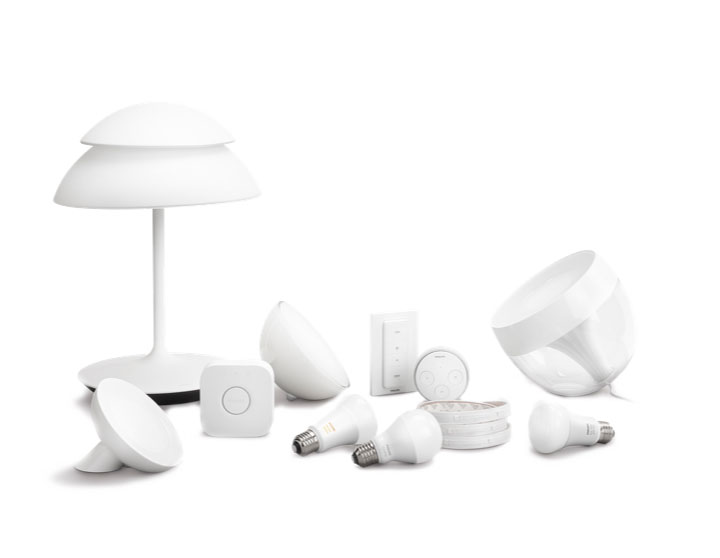
\includegraphics[height=6cm]{irodalom_res/philips_hue_termekek}
                    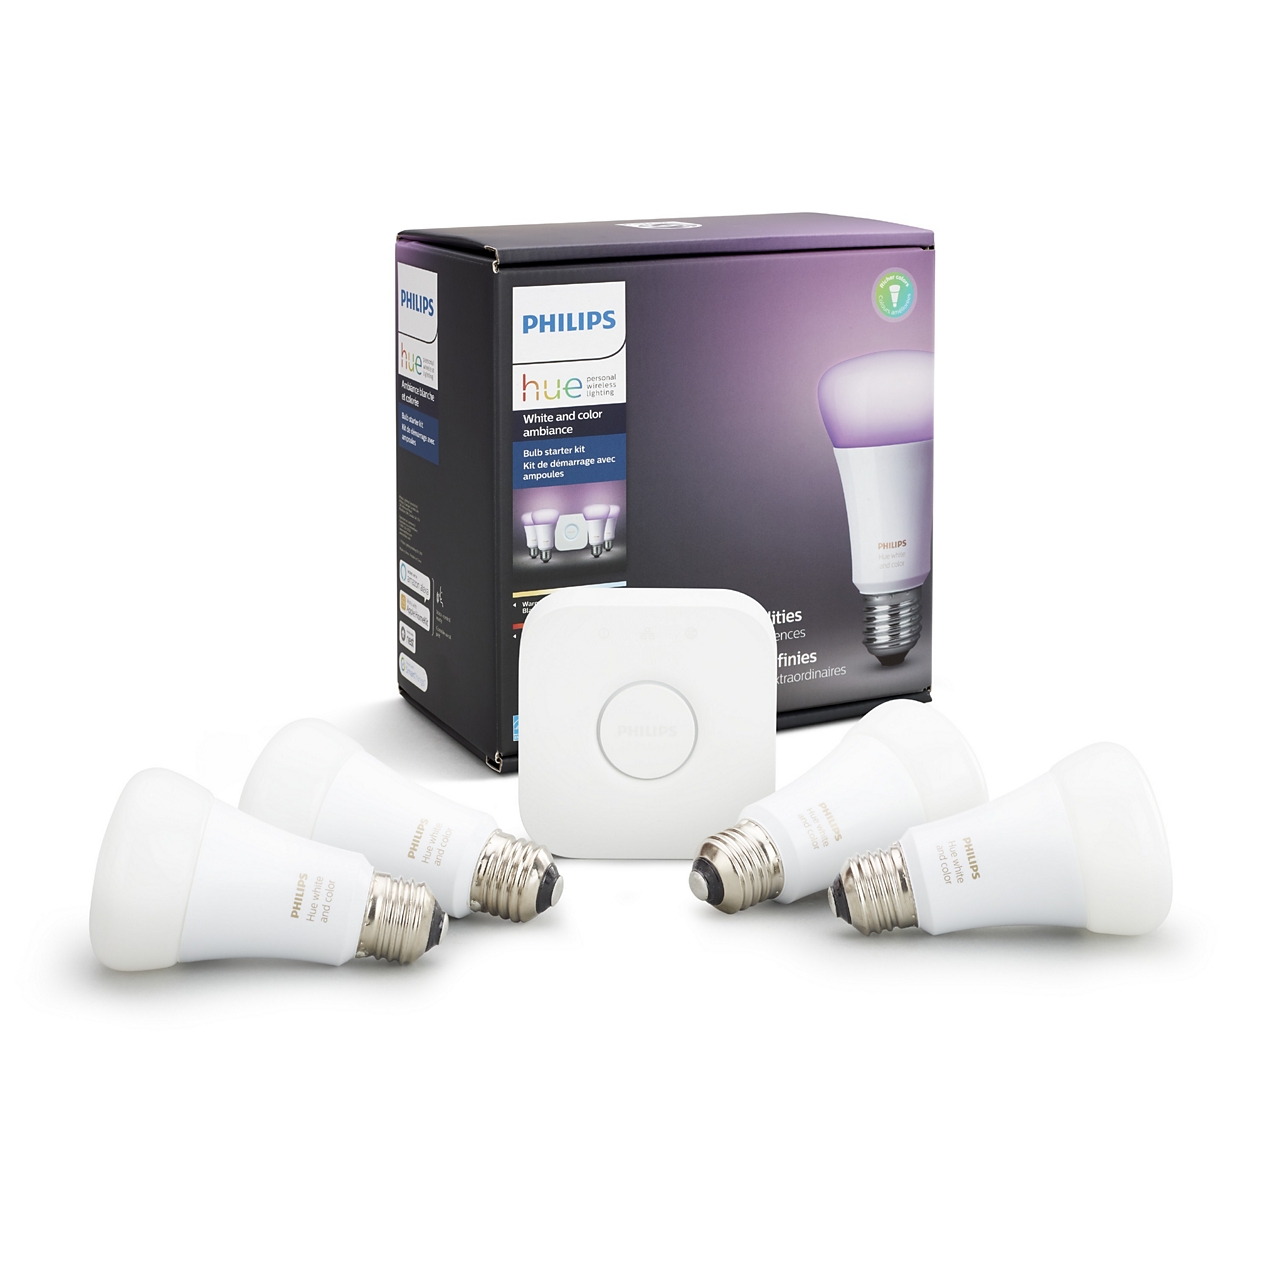
\includegraphics[height=6cm]{irodalom_res/philips_hue_termekek_2}
                \caption{Philips HUE eszközök\cite{led_lighting7}\cite{led_lighting8}}
                \label{fig:philips_hue}
             \end{figure}

            
            
       \subsubsection{LIFX}
            A LIFX egy okos világításra specializálódott cég. A Philips HUE termékektől annyiban különbözik, hogy ezek számára nem kell egy központi vezérlőegység, hanem képesek külön-külön működni. Egyedül a LED szalag és csempe termékükhöz kell külön vezérlőegység. Ez a termékcsalád is vezérelhető hanggal, támogatja továbbá a Google Asszisztenst, az Apple HomeKit-et, az Amazon Alexa-t és a Logitech Harmony rendszereket is. Árát tekintve hasonló kategóriába esik a Philips termékekkel. 
            
            \begin{figure}[h!]
                \centering
                    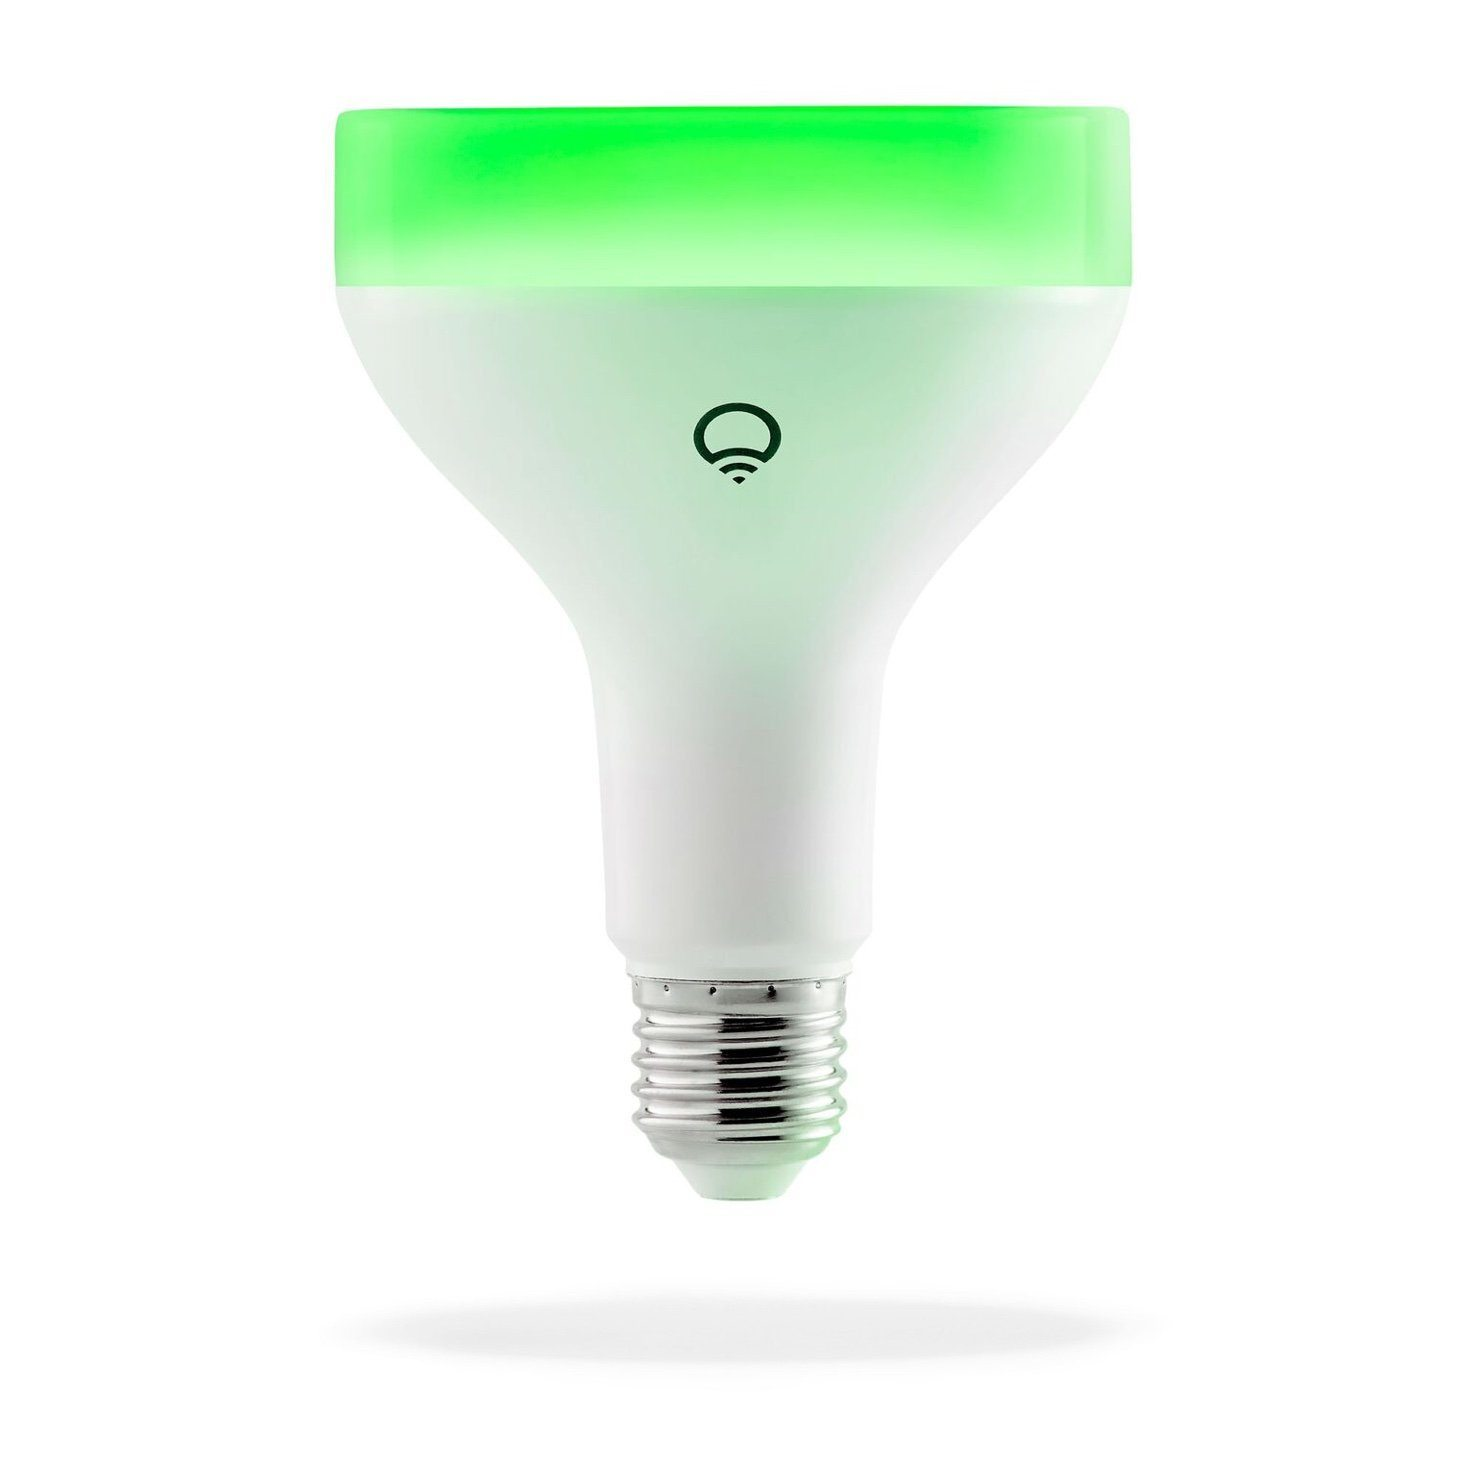
\includegraphics[height=6cm]{irodalom_res/LIFX_bulb}
                    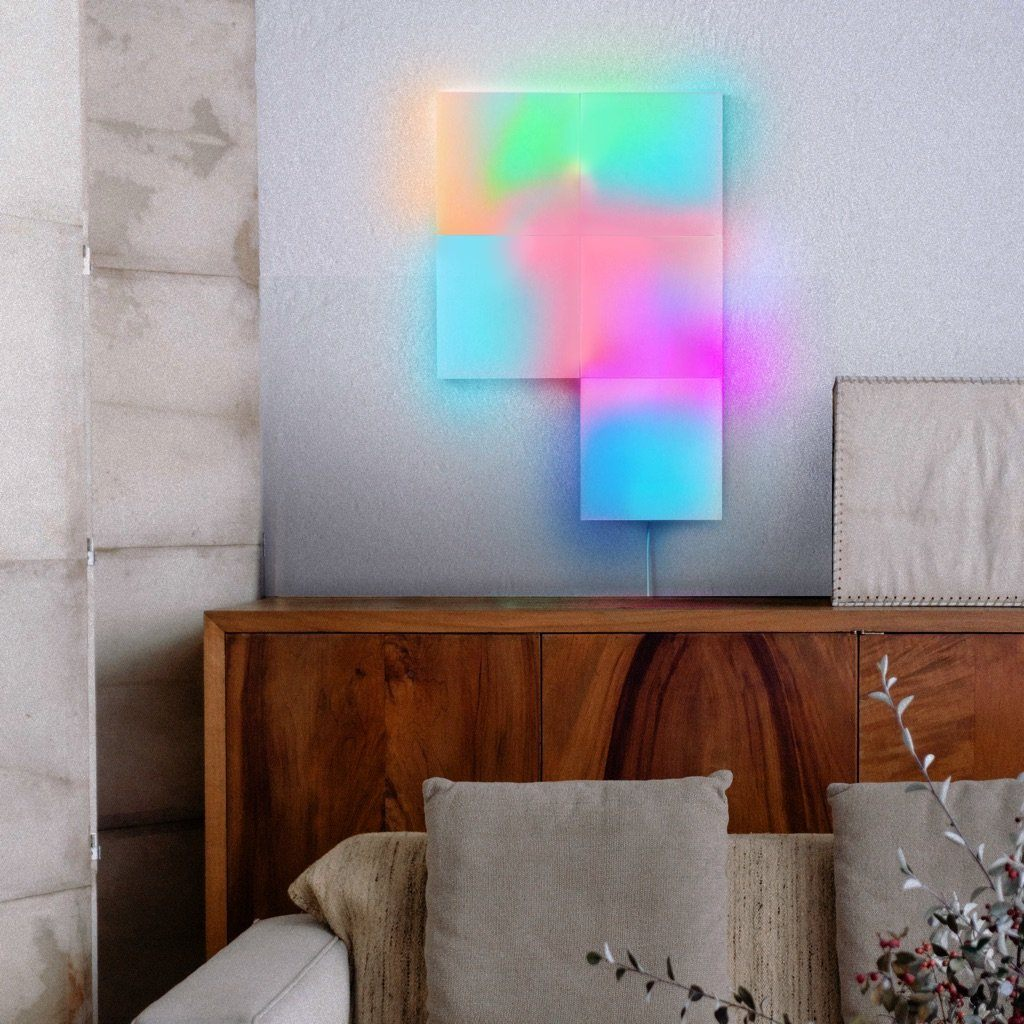
\includegraphics[height=6cm]{irodalom_res/LIFX_tile}
                    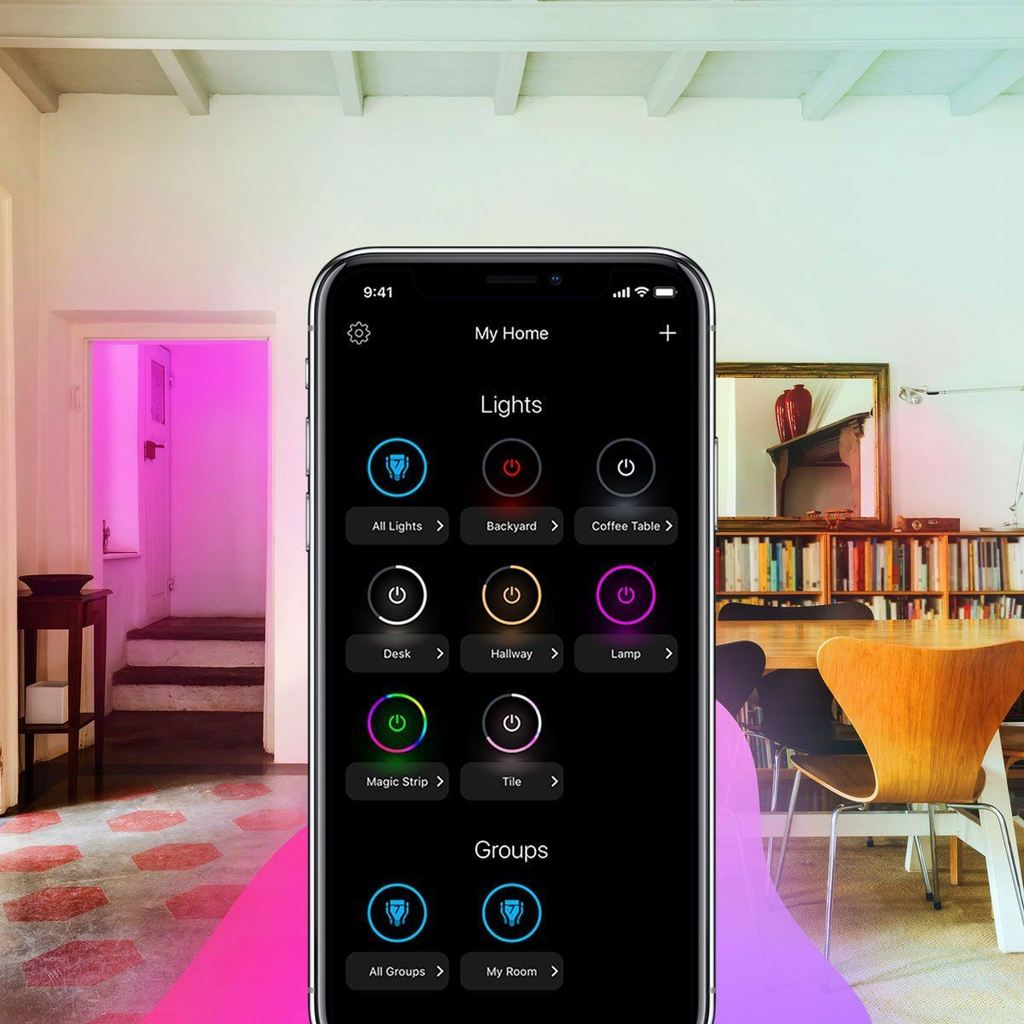
\includegraphics[height=6cm]{irodalom_res/LIFX_app1}
                    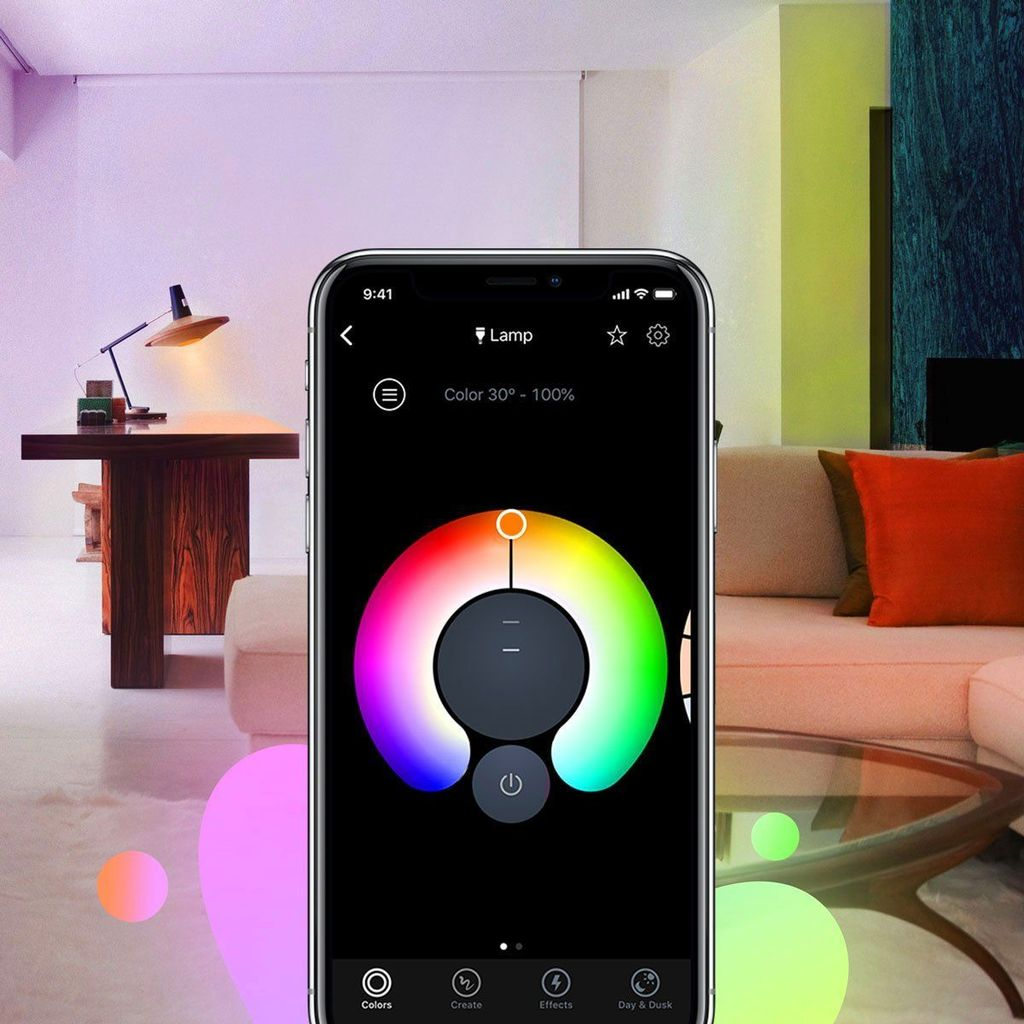
\includegraphics[height=6cm]{irodalom_res/LIFX_app2}
                \caption{LIFX termékek\cite{led_lighting9}\cite{led_lighting10}}
                \label{fig:lifx}
             \end{figure}
        
        \subsubsection{TP-Link okos villanykörte}
            A kedvező áru, vezeték nélküli hálózati eszközökről ismert TP-Link is forgalmaz okos villanykörtéket, illetve egyéb okos otthon megoldásokat. Az ár ez esetben is kedvező, habár a vevői visszajelzések nem olyan jók, mint az előző két termék esetében. A hangvezérlés Amazon Alexa-val és Google Asszisztenssel itt is támogatott.\cite{led_lighting11}
            \begin{figure}[h!] 
                \centering
                    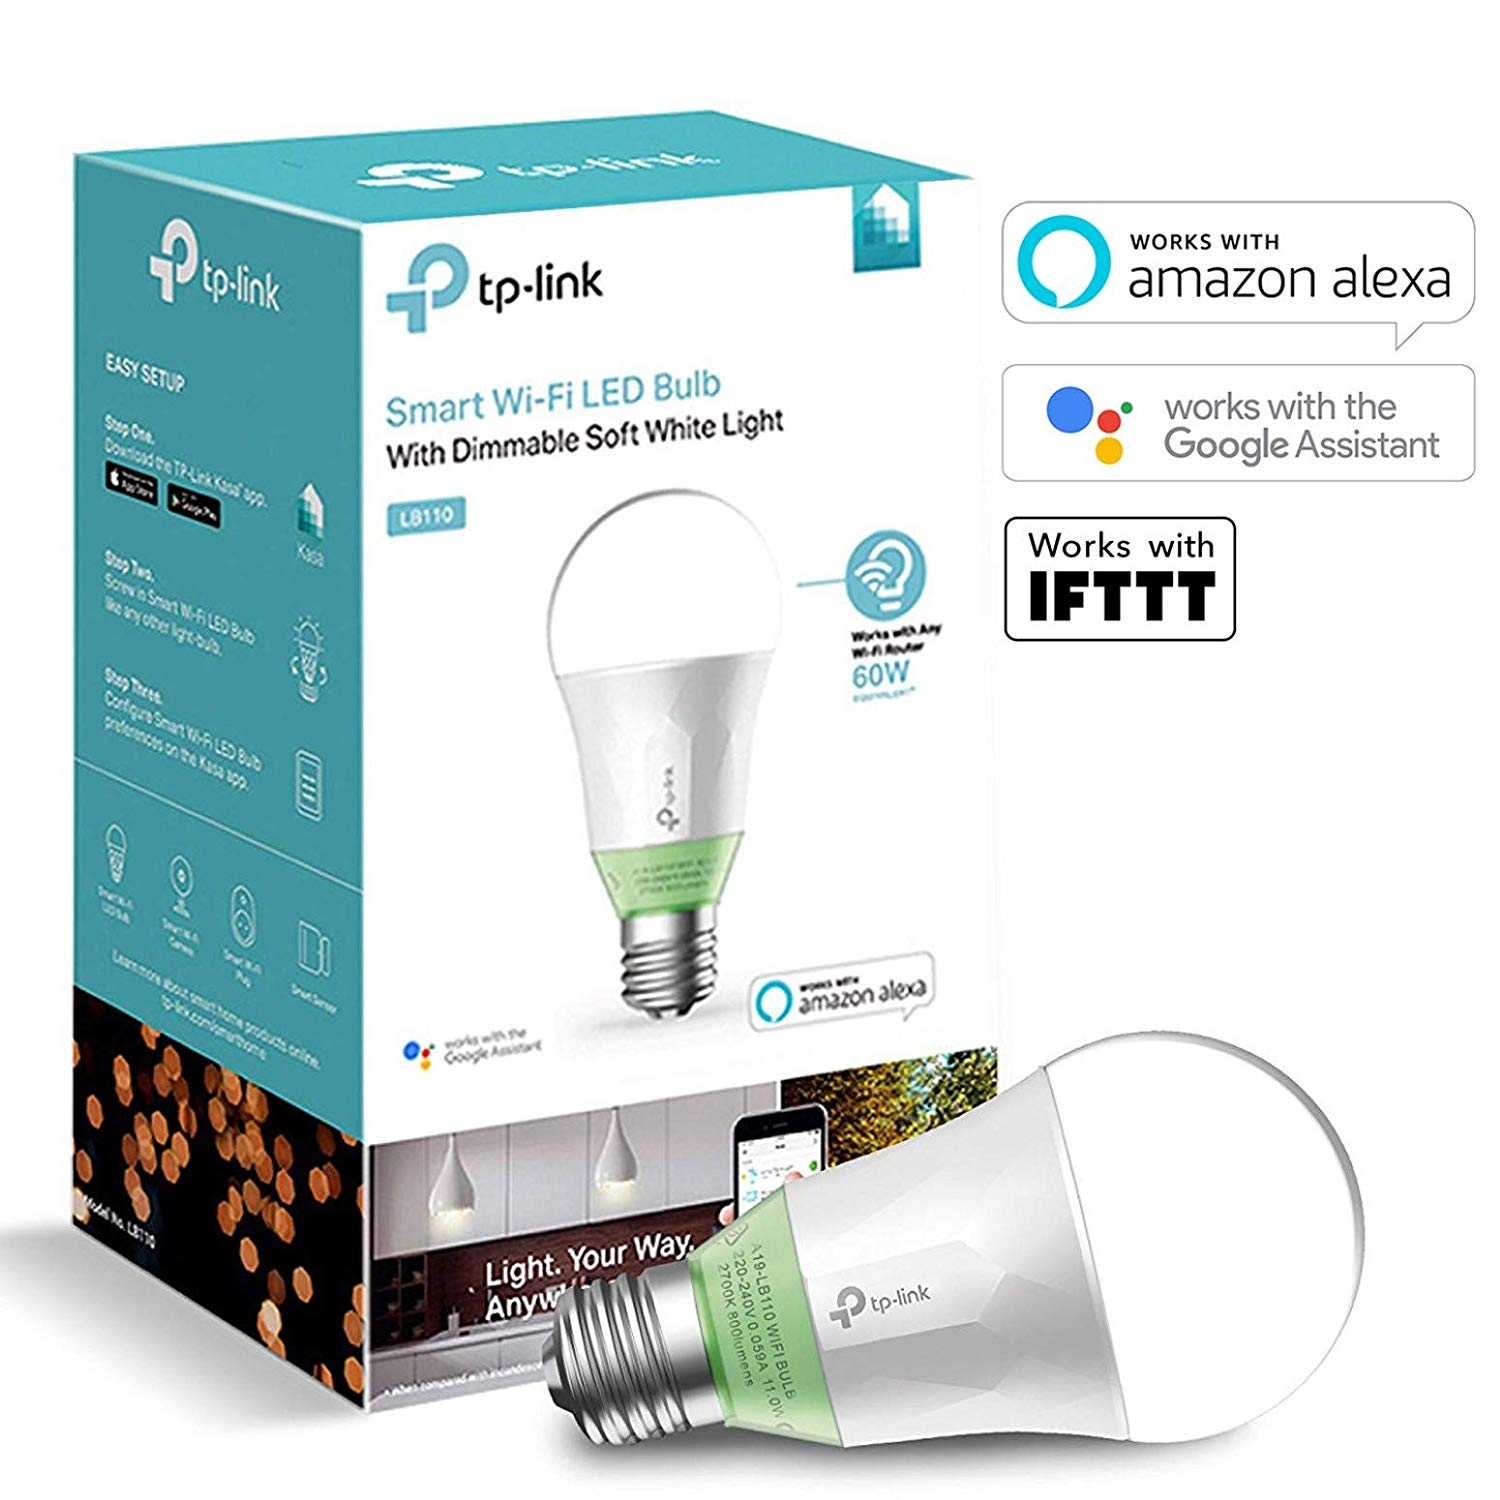
\includegraphics[height=6cm]{irodalom_res/tplink_bulb}
                \caption{TP-Link okosizzó\cite{led_lighting11}}
                \label{fig:tplink_bulb}
             \end{figure}
        
        \subsubsection{Általános vezérelhető LED szalag} 
            Talán a legolcsóbb LED-es világítások az Ebay-en, Amazon-on, Aliexpress-en, és hasonlókon rendelhető LED sorok. Ezeket többnyire áramforrással és egy egyszerűbb infrás távirányítóval működtethető vezérlőegységgel adják. Általában csak egy szín állítható be az egész szalagon, ellentétben a címezhető LED szalagokkal. \cite{led_lighting12}
            
            \begin{figure}[h!] 
                \centering
                    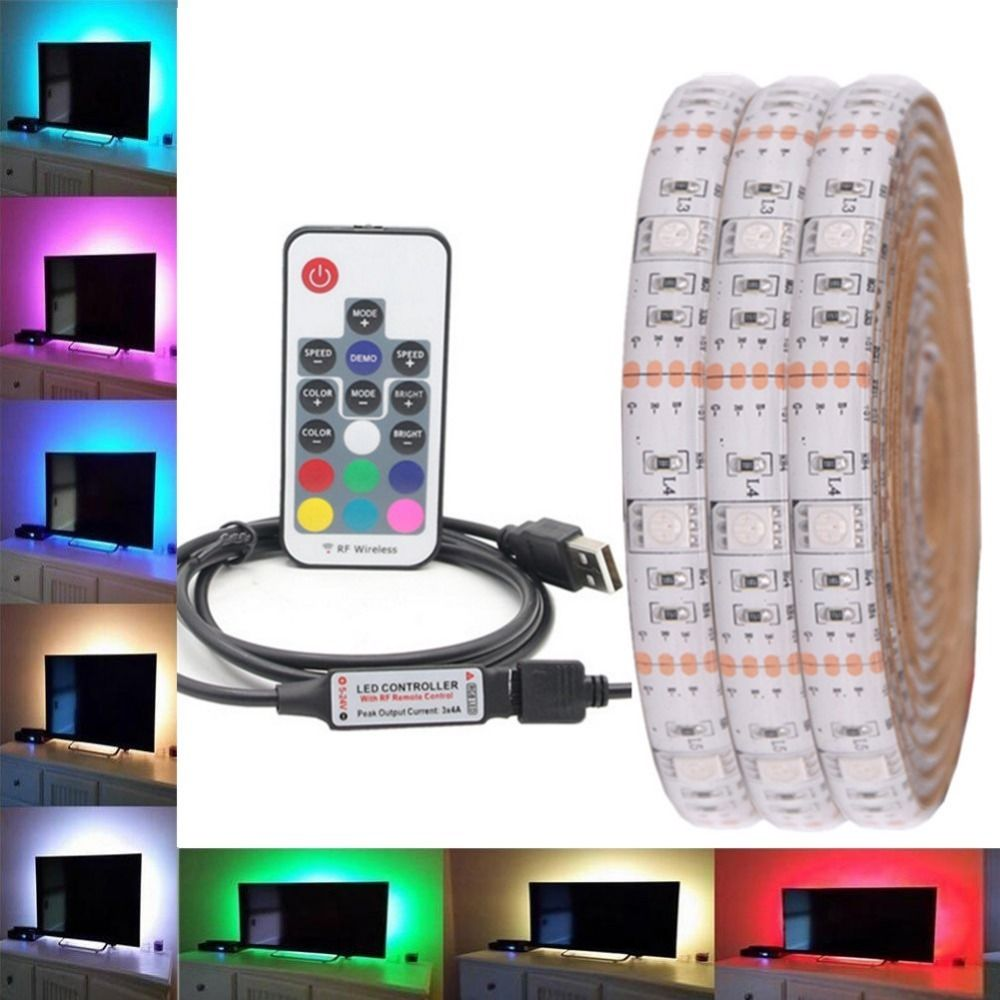
\includegraphics[height=6 cm]{irodalom_res/std_ledstrip}
                \caption{Általános LED szalag\cite{led_lighting12}}
                \label{fig:std_ledstrip}
             \end{figure}
        
\newpage

\end{document}

